\documentclass[edipack2.tex]{subfiles}
\begin{document}

\section{Examples}\label{SecExamples}
In this section we illustrate the functioning of the \NAME
library and their interfaces as solver for DMFT through specific examples, including
discussion of relevant code snippets. 


\subsection{Hubbard model on the Bethe lattice (Fortran API)}\label{SecExamplesBetheDMFT}
The test bed for any DMFT application is conventionally considered 
the description of the Mott or metal-to-insulator transition (MIT) 
in a Bethe lattice, i.e., a Cayley tree with coordination number 
$z\to\infty$~\cite{Georges1996}.
Here, we present a guided implementation of the DMFT 
solution for the Bethe lattice at $T=0$ using \NAME as impurity
solver.
The model under consideration is the Fermi-Hubbard Hamiltonian:
$$
H = -t \sum_{\langle ij\rangle,\s} c^\dagger_{i\s} c_{j\s} + 
    U \sum_i n_{i\up}n_{i\dw}
    $$
    
where $c^\dagger_{i\s}$ ($c_{i\s}$) are the creation (annihilation) 
operators for an electron at site $i$ with spin $\s$, and 
$n_{i\s} = c^\dagger_{i\s} c_{i\s}$ is the corresponding occupation 
operator. The first sum runs over nearest-neighbor pairs 
$\langle ij \rangle$.

The system is defined on a Bethe lattice with density of states
$\rho(\e)=\frac{1}{2D}\sqrt{D^2-\e^2}$,
where $D=2t$ is the half-bandwidth.
In DMFT this lattice model is mapped onto a quantum impurity problem with 
an effective electronic bath that must be determined
self-consistently.

Below, we present the key components of a basic DMFT implementation 
using \NAME for the Bethe lattice, employing either the Fortran or 
C++ APIs. Fully operational versions of the two codes can be found 
in the {\tt examples} directory of the \NAME source code. Both 
samples share a similar initial structure, including memory 
allocation, Bethe lattice creation, and solver initialization.

\setbox0=\hbox{%
  \begin{minipage}{0.465\linewidth}
    \center{\bf Fortran}
\begin{lstlisting}[style=fstyle,frame=none,numbers=none,basicstyle={\scriptsize\ttfamily}]
program ed_hm_bethe
   USE EDIPACK
   USE SCIFOR
   implicit none
   integer                :: Le=1000
   real(8)                :: wmixing=0.5d0
   real(8)                :: D=1d0
   integer                :: Nb
   real(8),allocatable    :: Bath(:)
   complex(8),allocatable :: Hloc(:,:,:,:)
   real(8),allocatable    :: Ebands(:),Dbands(:)
   complex(8),allocatable :: Smats(:,:,:,:,:)
   complex(8),allocatable :: Delta(:,:,:,:,:)
   ...  
   !Read variables
   call ed_read_input('inputED.conf')
   !Solver-specific arays
   allocate(Smats(Nspin,Nspin,Norb,Norb,Lmats))
   allocate(Delta(Nspin,Nspin,Norb,Norb,Lmats))
   allocate(Hloc(Nspin,Nspin,Norb,Norb));Hloc=0d0
   ...
   !Initialize Bethe arrays
   allocate(Ebands(Le),Dbands(Le))
   Ebands = linspace(-D,D,Le,mesh=de)
   Dbands = dens_bethe(Ebands,Wband)*de
   !Set local H
   call ed_set_hloc(Hloc)
\end{lstlisting}
\end{minipage}
}
\savestack{\listingA}{\box0}

\setbox0=\hbox{%
  \begin{minipage}{0.505\linewidth}
    \center{\bf C++}
\begin{lstlisting}[style=cstyle,frame=none,numbers=none,basicstyle={\scriptsize\ttfamily}]
#include <edipack_cbindings.h>
using namespace std;
...
//Main variables
int Le = 1000;
int iloop = 0;
double wmixing = 0.5;
double D = 1.0;
//Read  variables    
char input[] = "inputED.conf"; 
read_input(input);      
//Dimensions
int64_t d[4] = {Nspin,Nspin,Norb,Norb};
int total_size = d[0] * d[1] * d[2] * d[3];
int total_size_n5 = total_size * Lmats;    
// Solver-specific arrays
vector<complex<double>> Hloc(total_size);
vector<complex<double>> Smats(total_size_n5);
vector<complex<double>> Delta(total_size_n5);
...
// Initialize Bethe arrays
vector<double> Ebands, Dbands;
Ebands = linspace(-D,D,Le);
Dbands = dens_bethe(Ebands,Wband,de);
//set local H
ed_set_Hloc_single_N4(Hloc.data(), d);
\end{lstlisting}
\end{minipage}
}
\savestack{\listingB}{\box0}

\begin{tabular}{c|c}\label{list2}
  \stackinset{l}{}{t}{}{}{\listingA} & \stackinset{l}{}{t}{}{}{\listingB} 
\end{tabular}

The bath is described by the (unknown) function $\GG^{-1}_0$, known as 
the Weiss field ({\tt Weiss}). In the ED approach implemented in \NAME, 
the bath is approximated using a finite number of discrete energy levels. 
The function $\GG^{-1}_0$ is then used to determine the bath parameters 
$\vec{x} = \{V, h\}$ through the optimization method outlined in 
\secu{sSecFit}.

The starting point for any calculation is a reasonable initial guess 
for the Weiss field, or equivalently, the bath parameters. In \NAME, 
this is accomplished using the function {\tt
  ed\_init\_solver} (Fortran API) or {\tt init\_solver\_site} (C++ API).

\setbox0=\hbox{%
  \begin{minipage}{0.465\linewidth}
    \center
    \begin{lstlisting}[style=fstyle,frame=none,numbers=none,basicstyle={\scriptsize\ttfamily}]
   !Initialize solver
   Nb=ed_get_bath_dimension()
   allocate(bath(Nb))
   call ed_init_solver(bath)
\end{lstlisting}
\end{minipage}
}
\savestack{\listingA}{\box0}

\setbox0=\hbox{%
  \begin{minipage}{0.505\linewidth}
    \center
\begin{lstlisting}[style=cstyle,frame=none,numbers=none,basicstyle={\scriptsize\ttfamily}]
// Initialize solver
int Nb;
vector<double> Bath(Nb);
Nb = get_bath_dimension();
int64_t bath_dim[1] = {Nb};
init_solver_site(Bath.data(), bath_dim);
\end{lstlisting}
\end{minipage}
}
\savestack{\listingB}{\box0}

\begin{tabular}{c|c}\label{list2}
  \stackinset{l}{}{t}{}{}{\listingA} & \stackinset{l}{}{t}{}{}{\listingB} 
\end{tabular}


The iterative algorithm to solve the DMFT problem is based on
a reverse communication strategy and proceeds as follows:
\begin{itemize}
  
\item[{\tiny $\blacksquare$}] Call the exact diagonalization {\bf impurity solver}
  whose only input is the set of parameters $\vec{x}$ contained in a
  rank-1 array. All  \NAME options are controlled through input file
  specifications.
  
\item[{\tiny $\blacksquare$}] Retrieve the self-energy functions $\Sigma_{\a\b\s\s'}(i\omega)$ on the
  Matsubara axis using dedicated function provided by \NAME API.
  
\item[{\tiny $\blacktriangleright$}] Evaluate the local interacting Green's function
  $G_\mathrm{loc}(i\omega) = \int_{-D}^D \frac{\rho(\e)}{\zeta -\e}d\e$ with
  $\zeta=i\omega+\mu-h^0-\Sigma(i\omega)$.
  
\item[{\tiny $\blacktriangleright$}] Update the Weiss field via the {\bf self-consistency}
  relation: $\GG^{-1}_0(i\omega) = G_\mathrm{loc}(i\omega) +
    \Sigma(i\omega)$. For the Bethe lattice, this simplifies to
    $\Delta = \tfrac{D}{4}G_\mathrm{loc}$.
    
  \item[{\tiny $\triangleright$}] Optimize the bath parameters $\vec{x}$ against the updated
    Weiss field,  potentially using the conjugate gradient procedures 
supplied by \NAME. Then, restart at step 1.
\end{itemize}

The first two steps, marked by the ${\tiny \blacksquare}$ symbol, 
are handled directly by \NAME routines. In the subsequent steps, 
indicated by the ${\tiny \blacktriangleright}$ symbol, control returns 
to the user, who must implement the algebraic updates required to 
close the self-consistency loop and optimize the bath.
Given the 
critical importance of this optimization, \NAME provides access to 
well-tested functions, ensuring stability and reproducibility of 
results. Alternative optimization methods can also be employed as 
needed. 
An example of implementation is provided in the following listings.


\setbox0=\hbox{%
  \begin{minipage}{0.45\linewidth}
    \center
    \begin{lstlisting}[style=fstyle,frame=none,numbers=none,basicstyle={\scriptsize\ttfamily}]
!DMFT loop
do while(.not.converged.AND.iloop<nloop)
    iloop=iloop+1     
    ! Call ED Solver
    call ed_solve(bath)     
    ! Retrieve Self-energy on Matsubara axis
    call ed_get_sigma(Smats,'m')
    ! Build local Green's function
    wfreq = pi/beta*(2*arange(1,Lmats)-1)
    do i=1,Lmats
       zeta= xi*wfreq(i)+xmu - Smats(1,1,1,1,i)
       Gmats(1,1,1,1,i)=sum(DOS/(zeta-Ene))*de  
    enddo
    ! Self-consistency
    Delta = D/4d0*Gmats
    ! Fitting -> new bath
    call ed_chi2_fitgf(Weiss,bath,ispin=1)     
    ! Check convergence
    converged=check_convergence(Delta,&
          dmft_error,Nsuccess,Nloop)
enddo
\end{lstlisting}
\end{minipage}
}
\savestack{\listingA}{\box0}

\setbox0=\hbox{%
  \begin{minipage}{0.52\linewidth}
    \center
\begin{lstlisting}[style=cstyle,frame=none,numbers=none,basicstyle={\scriptsize\ttfamily}]
  // DMFT loop
  while (iloop < Nloop && !converged) {
    //  Call ED Solver
    solve_site(Bath.data(),bath_dim,1,1);      
    // Retrieve  Self-energy on Matsubara axis
    get_sigma_site_n5(Smats.data(),//
        0,0,wm.data(),Lmats,0);
    //  Build a local Green's function:
    for (int i=0;i<Lmats;++i) {
      zeta= wm[i] + xmu - Smats[i];
      Gmats[i] = complex<double>(0.0,0.0);
      for (int j=0; j< Le; j++) {
        Gmats[i]+=Dbands[j]/(zeta-Ebands[j]);
      }
    }
    // Self-consistency
    for (int i = 0; i < Lmats; ++i) {
      Delta[i] = 0.25 * D * Gmats[i];
    }
    // Fit -> new bath
    chi2_fitgf_single_normal_n5(Delta.data(),//
        delta_dim,Bath.data(),bath_dim,1,0,1);
    // Check convergence
    converged = check_convergence(Delta,//
        dmft_error, Nsuccess, Nloop, comm);  
  }
\end{lstlisting}
\end{minipage}
}
\savestack{\listingB}{\box0}

\begin{tabular}{c|c}\label{list2}
  \stackinset{l}{}{t}{}{}{\listingA} & \stackinset{l}{}{t}{}{}{\listingB} 
\end{tabular}




\paragraph{Results}
In the following, we present results for the interaction-driven Mott 
transition in the Bethe lattice, which captures the gradual 
transformation of a partially-filled metallic state into a correlated 
insulator.
To illustrate this, we report in panel (A) the evolution of the spectral 
function $-{\rm Im}G_\mathrm{loc}(\omega)/\pi$ as a function of the 
interaction strength $U$. Despite the inherently {\it spiky} nature 
of the spectrum, resulting from the finite number of poles in the 
discretized effective bath, the characteristic features of the Mott 
transition are clearly visible. At low energies, a renormalized 
quasi-particle peak develops at the Fermi level ($\omega = 0$). 
Simultaneously, the system exhibits the formation of incoherent 
high-energy features, which eventually evolve into well-defined 
Hubbard bands in the Mott insulating phase for $U > U_\mathrm{c}$, 
with $U_\mathrm{c} \simeq 2.8D$.

\begin{figure}[t!]
  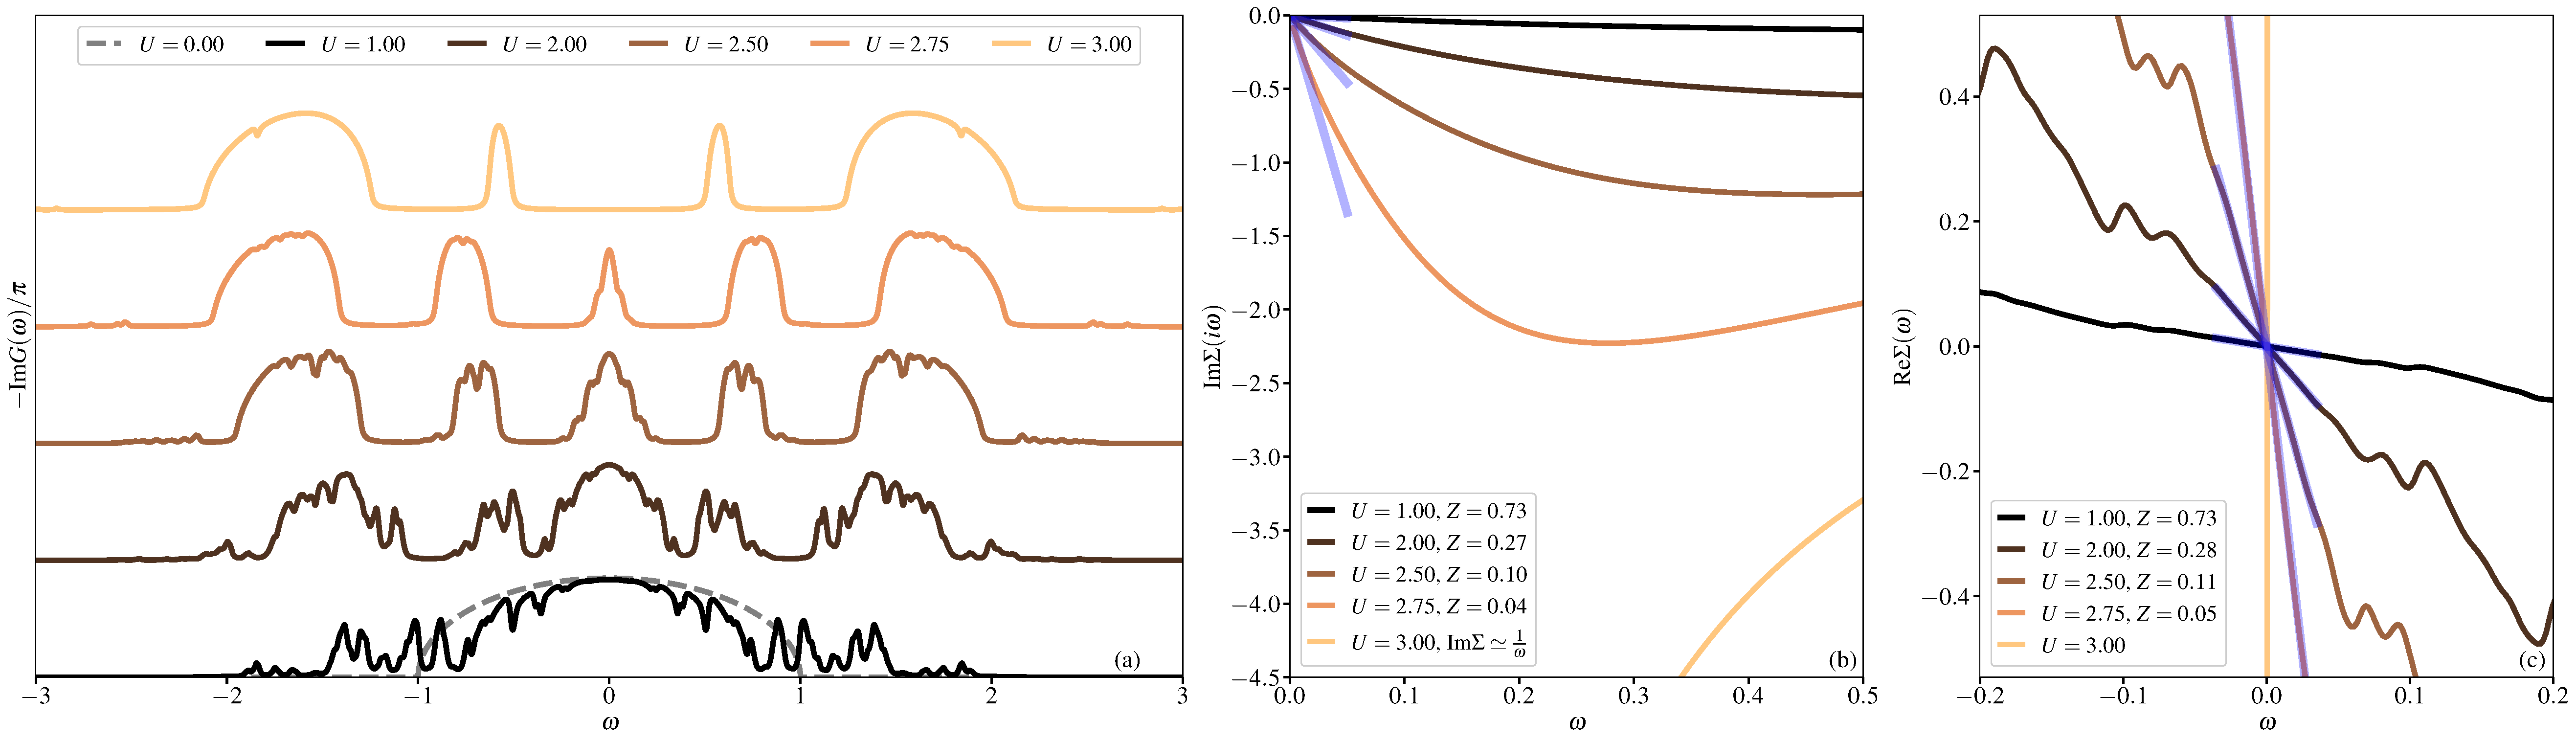
\includegraphics[width=\linewidth]{figures/figBethe.pdf}
    \caption{\label{figEx1}%
      \textbf{The Metal-Insulator Mott transition.}
      (a) Evolution of the spectral function $-\Im{G}(\omega)/\pi$ as
      a function of increasing interaction $U$. The critical
      interaction $U_\mathrm{c}\simeq 2.8D$ separates the correlated metal $U<U_\mathrm{c}$ from
      the Mott insulator $U>U_\mathrm{c}$.
      (b)-(c) The corresponding evolution of the Matsubara self-energy
      $\Im\Sigma(i\omega)$ (b) and
      real-axis one $\Re\Sigma(\omega)$ across the Mott
      transition. For a particle-hole symmetric case both allow to
      estimate the renormalization constant $Z$ (see main text), using
      linear order expansion in frequency (blue solid lines). The
      values of $Z$ are reported in the legend.
      The Mott insulating solution is associated to a singularity at
      $\omega=0$ of $\Im\Sigma$. 
        }
\end{figure}

The formation of a spectral gap separating the Hubbard bands in the 
Mott insulating phase is associated with the divergence of the 
imaginary part of the self-energy at the Fermi level. This divergence 
reflects the complete localization of the electrons, effectively 
suppressing coherent quasi-particle excitations. Specifically, 
causality dictates that the real part of the self-energy must also 
grow significantly near the singularity, making it impossible to 
satisfy the quasi-particle pole equation
$$
\omega+\mu-h^0-\e-\Re{\Sigma}(\omega)=0,
$$
which governs the formation of coherent excitations near the Fermi 
level.

Panels (B) and (C) illustrate this phenomenon by showing the evolution 
of the self-energy $\Sigma$. In panel (B), we present the Matsubara 
self-energy ${\rm Im}\Sigma(i\omega)$ in the low-energy regime. As the 
interaction strength $U$ increases, this function progressively 
grows, eventually diverging as the critical interaction threshold 
$U > U_\mathrm{c}$ is crossed.
This divergence along the Matsubara axis is directly linked to the
particle-hole symmetry of the Bethe lattice, which pins the  ${\rm
  Im}\Sigma$ singularity at $\omega = 0$.

Panel (C) complements this picture by displaying the real part 
$\Re{\Sigma}(\omega)$ in the same low-energy regime. Here, increasing 
$U$ leads to a rapid rise of this component, culminating in a 
discontinuous behavior as the critical point is approached. This 
discontinuity directly reflects the divergence in the imaginary part
on the real-axis,  confirming the transition to the Mott insulating state.


A quantitative measure of this transition is provided by the 
quasi-particle renormalization factor $Z$, which can be used to capture the degree 
of electron delocalization. This parameter ranges from 1 for a 
non-interacting metal to 0 for a fully localized Mott insulator. It is 
defined through the low-energy expansion of the self-energy as
$$
Z=(1-\tfrac{\partial\Re\Sigma}{\partial\omega}_{|_{\omega\rightarrow
    0}})^{-1}.
$$
which can also be estimated from the linear behavior of ${\rm Im}\Sigma(i\omega)$ for 
$\omega\to0$ in the metallic regime using the relation:
$$
   \frac{\Im\Sigma(i\omega_n)}{\omega_n}_{|_{\omega_n\rightarrow 0}}=
   \frac{1}{\pi}\int_{\mathbb R}d\epsilon \frac{\Re\Sigma(\epsilon)}{\epsilon^2}=
   \frac{\partial\Re\Sigma}{\partial\omega}_{|_{\omega\rightarrow 0}}.
$$

The linear fits highlighted in panels (B) and (C), along with the 
corresponding $Z$ values provided in the legends, clearly indicate that 
the slope of the self-energy at low energy increases with $U$ on both 
the Matsubara and real axes. At the transition point, this slope 
diverges, reflecting the onset of complete electron localization as 
$Z \to 0$, consistent with the divergence 
${\rm Im}\Sigma(\omega) \rightarrow -\infty$.






\subsubsection{Finite temperature solution (w2dynamics interface)}\label{SecExamplesBetheDMFTw2d}
To demonstrate the usage of the w2dynamics interface to \NAME,  here we briefly discuss how to solve the same problem, i.e. the Hubbard model on the Bethe lattice within DMFT using w2dynamics. 
In order to showcase the capabilities of \NAME to address low-temperature problems we compare the continuous-time Quantum Monte Carlo (CTQMC) solver using the hybridization expansion method (CT-HYB) included in w2dynamics against the \NAME solver at finite temperature.  

In contrast to the \NAME API that only enables access to the impurity solver and bath optimization procedures, but requires the user to implement (using different methods) the DMFT algorithm themselves, the standard way to use w2dynamics is fundamentally different: a single Python script {\tt DMFT.py} is provided that takes care of the whole DMFT calculation via dedicated classes to implement generic self-consistency. The w2dynamics calculation is then entirely controlled by a model-dependent parameters file {\tt Parameters.in}, which contains a number of variable specifications including options to control the ED solver inherited from \NAME. Further information about the functioning of w2dynamics can be found in Ref.~\onlinecite{Wallerberger2019CPC}           

Another important difference concerns the initial point of the iterative DMFT solution algorithm: while \NAME starts from a given discrete bath, w2dynamics is initialized with a zero self-energy function or alternatively reads this quantity from a converged solution file. When using the \NAME ED interface, the initial Weiss field is determined using self-consistency and finally an initial discrete bath is obtained through the \NAME bath optimization procedure. 

The w2dynamics configuration file for the solution of the Bethe lattice problem at finite temperature reads: 
\begin{lstlisting}[style=mybash,language={},numbers=none,basicstyle={\scriptsize\ttfamily}]
[General]
DOS             = Bethe           # support for the Bethe lattice is built-in
half-bandwidth  = 1               # list of half-bandwidths per orbital
NAt             = 1               # number of impurities
beta            = 100             # inverse temperature
mu              = 1.0             # chemical potential set to achieve half-filling
EPSN            = 0.0             # turns off filling-based chemical potential search
DMFTsteps       = 100             # given no convergence checking, we might want fewer
magnetism       = para            # symmetrize self-energies per spin
FileNamePrefix  = bethe_dmft_U2   # prefix for the output file name
fileold         = bethe_dmft*hdf5 # file to read an initial self-energy from
readold         = 0               # iteration number to read initial self-energy from, 0 turns off
mixing          = 0.5             # mixing, but mixes self-energies and not Weiss fields
mixing_strategy = linear          # linear mixing as in the Fortran example
FTType          = none            # (for CT-HYB): use the NFFT-measured G
solver          = EDIPACK         # use EDIpack as impurity solver, not default CTHYB

[Atoms]
[[1]]                             # one subsection per impurity
Nd              = 1               # number of orbitals
Hamiltonian     = Kanamori        # create a Hubbard-Kanamori interaction Hamiltonian
Udd             = 2.0             # equivalent to ULOC
Vdd             = 1.0             # equivalent to UST, meaningless for 1 orbital
Jdd             = 0.5             # equivalent to JH, JX and JP, also meaningless here

[EDIPACK]                         # further ED parameters, as in the Fortran example
NBATH           = 7               # number of bath sites
ED_TWIN         = True            # use twin symmetry
LFIT            = 2048            # number of Matsubara frequencies used for the bath fit
LANC_NGFITER    = 500             # number of Lanczos iterations for Green's function
CG_FTOL         = 1e-10           # conjugate-gradient tolerance
CG_NITER        = 2048            # maximum number of conjugate-gradient iterations
ED_FINITE_TEMP  = True            # at finite temperature T = 1/beta

[QMC]                             # Parameters for some grid sizes and the CT-HYB calculation
Ntau            = 1024            # imaginary time grid size
Niw             = 4096            # number of positive Matsubara frequencies
# parameters only relevant for CT-HYB follow
MeasGiw         = 1               # enable NFFT measurement of G
NCorr           = 175             # estimate of the autocorrelation length
Nmeas           = 200000          # number of measurements / sample size
Nwarmups        = 1000000         # number of initial warmup steps for Markov chain thermalization
\end{lstlisting}
Assuming that w2dynamics is installed to {\tt /opt/w2dynamics} and the preceding parameters file saved as {\tt bethe\textunderscore{}dmft.in}, we can start the calculation by running the {\tt DMFT.py} script:
\begin{lstlisting}[style=mybash,numbers=none]
mpiexec -n 10 /opt/w2dynamics/DMFT.py bethe_dmft.in
\end{lstlisting}

The results are collected into an HDF5 archive in the usual w2dynamics format, including output quantities inherited from \NAME. Results can be viewed using the script {\tt hgrep} provided with w2dynamics or with other HDF5 tools. In this example we extract the Matsubara self-energy function $\Sigma(i\omega_n)$ for the last DMFT iteration:
\begin{lstlisting}[style=mybash,numbers=none]
/opt/w2dynamics/hgrep latest siw-full -1
\end{lstlisting}

\begin{figure}%[t!]
  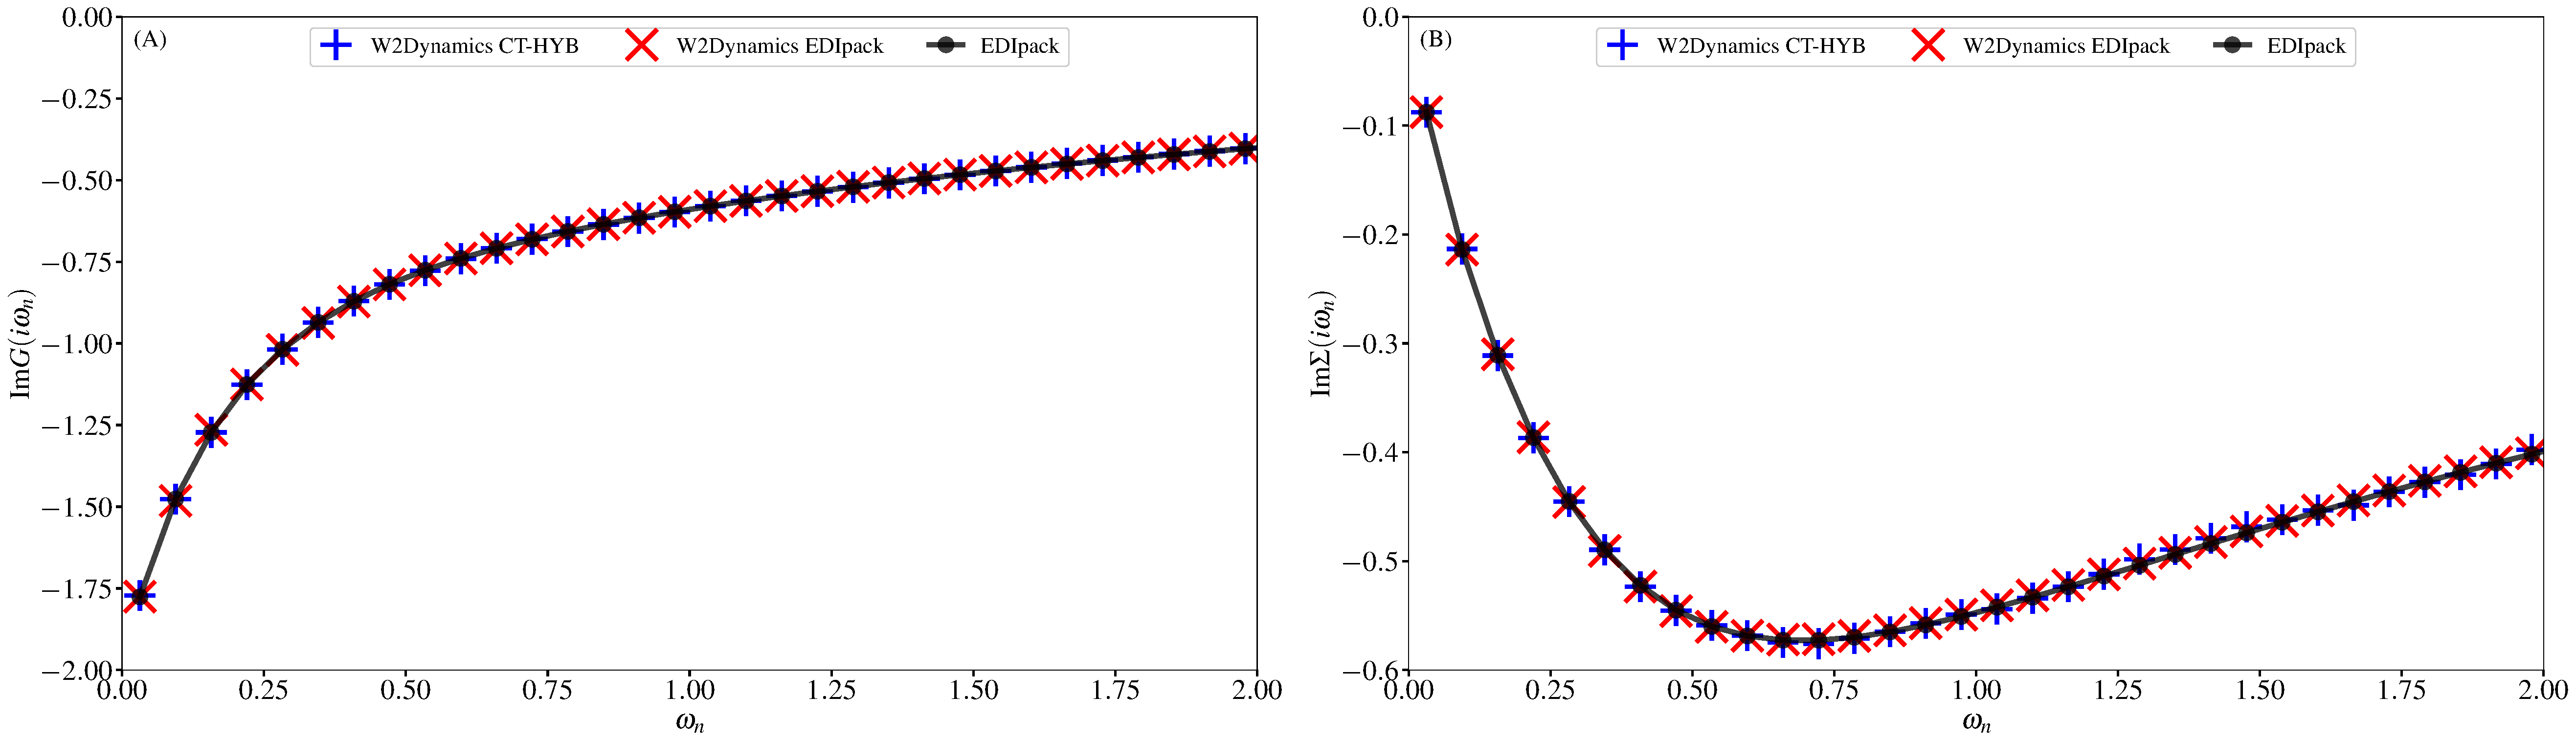
\includegraphics[width=\linewidth]{figures/figBetheW2D.pdf}
    \caption{\label{figEx1W}%
    \textbf{Finite temperature DMFT solution.}
    Comparison of the imaginary parts of the Green's function $\Im{G}(i\omega_n)$ and Self-energy $\Im{\Sigma}(i\omega_n)$ from different solutions of the Hubbard model on the Bethe lattice using DMFT. Data are for $T/D=0.01$ and $U/D=2.0$. CTQMC results from the solver included with w2dynamics are compared against \NAME ED results, used both through the w2dynamics interface and with a standalone Fortran program. 
        }
\end{figure}

In \figu{figEx1W} we report a comparison of the results obtained using the hybridization expansion CTQMC solver in w2dynamics and using the \NAME ED method both as a solver in w2dynamics and with a program using the Fortran API directly as shown in the previous subsection. Using DMFT, we solve the Hubbard model on a Bethe lattice for $T/D=0.01$ and $U/D=2.00$, corresponding to a correlated metallic state. 
In panel (A) we show the behavior of the imaginary part of the impurity Green's function $\Im{G}(i\omega_n)$ (note that w2dynamics does not directly have access to the real-axis Green's function when using the CTQMC solver). In panel (B) we show the same comparison for impurity self-energy $\Im{\Sigma}(i\omega_n)$. 
The results obtained from the three calculations are in this case nearly identical already for a small number of bath levels ({\tt NBATH=7}) and relatively low QMC statistics.   



















\subsection{Attractive Hubbard model (Python API, {\tt ed\_mode=superc})}\label{SecExamplesAHM}
The second example we present concerns the DMFT description of the 
attractive Hubbard model on a two-dimensional square lattice. This 
example has a twofold aim: (i) to demonstrate the support of \NAME 
for ($s$-wave) superconductivity, and (ii) to illustrate the use of 
the library's Python API through a concrete working example. The 
model Hamiltonian is given by:
$$
H = \sum_{\ka,\s} \epsilon(\ka) c^\dagger_{\ka\s} c_{\ka\s} 
    - U \sum_i n_{i\up} n_{i\dw},
$$
where $U > 0$, $c^\dagger_{\ka\s} = \tfrac{1}{\sqrt{N}} 
\sum_i e^{-i\ka \cdot R_i} c^\dagger_{i\s}$, and $c^\dagger_{i\s}$ 
is the creation operator for an electron at site $i$ with spin $\s$. 
The occupation operator is $n_{i\s} = c^\dagger_{i\s} c_{i\s}$, and 
the energy dispersion relation is $\e(\ka)=-2t[\cos{(k_x a)}+
\cos{(k_y a)}]$, where we set the lattice spacing 
$a=1$  and the choose the energy unit such as $4t=D=1$ for convenience.

The DMFT workflow for this case is largely similar to the previous 
example, but it now operates in the Nambu basis defined by the spinor
$$
\psi_i=\begin{bmatrix} c_{i\up} \\ c^\dagger_{i\dw} \end{bmatrix}. 
$$
In this basis, the Green's function takes the matrix form:
\begin{equation}
  {\mathbf G} =
  \begin{pmatrix}
    \hat{G}_{\uparrow\uparrow} & \hat{F}_{\uparrow\downarrow}\\
    \hat{\bar{F}}_{\downarrow\uparrow}  &    \hat{\bar{G}}_{\downarrow\downarrow} \\
  \end{pmatrix}
\end{equation}
where the symbol $\hat{A}$ indicates the potential multi-orbital 
nature of the system, which reduces to a scalar in the present 
single-orbital case. The components in the second row, denoted 
by $\hat{\bar{A}}$, are connected to the first row by particle-hole 
and time-reversal symmetries. The specific relations depend on the 
symmetry of the order parameter (here, $s$-wave) and whether the 
functions are defined on the Matsubara or real-frequency axis:
\begin{equation}
\begin{array}{cc}
  \hat{\bar{G}}(i\omega) = -\hat{G}^*(i\omega)\;; &  \hat{\bar{F}}(i\omega) = \hat{F}(i\omega)\\
  \hat{\bar{G}}(\omega)  = -\hat{G}^*(-\omega) \;; & \hat{\bar{F}}(\omega) = \hat{F}^*(i\omega)\\
\end{array}
\end{equation}  

The code implementation closely follows the structure of the previous 
example, with some notable adjustments related to the Nambu basis. 
Specifically, the above symmetries allow one to compute only the 
independent components from the first row, significantly reducing 
the computational effort. The initial part of the code handles the 
lattice structure and solver initialization, as described below.

\begin{lstlisting}[style=mypython,numbers=none,basicstyle={\scriptsize\ttfamily}]
import numpy as np
from edipy2 import global_env as ed
import mpi4py
from mpi4py import MPI
import os,sys
from aux_funx import * #include function to build $G_\mathrm{loc}$ 
comm = MPI.COMM_WORLD
rank = comm.Get_rank()
master = (rank==0)
#Functions
def generate_kgrid(Nk):
    b1=2*np.pi*np.array([1.0,0.0])
    b2=2*np.pi*np.array([0.0,1.0])
    n1, n2 = np.meshgrid(np.arange(Nk), np.arange(Nk))
    n1=n1/Nk;n2=n2/Nk
    gridout = np.stack([n1.ravel(), n2.ravel()], axis=-1)
    return np.dot(gridout,[b1,b2])
def h_square2d(k,t):
  return -2*t*(np.cos(k[...,0,np.newaxis,np.newaxis])+np.cos(k[...,1,np.newaxis,np.newaxis]))*np.eye(ed.Norb)
    
#Read input
ed.read_input("inputAHM.conf")

#Generate Hk and  set Hloc
kgrid = generate_kgrid(Nk)
Hk   = h_square2d(kgrid,t_hop)
HkNambu   = np.array([h_square2d(kgrid,t_hop),-np.conj(h_square2d(-kgrid,t_hop))])
Hloc = np.sum(Hk,axis=0)/Nk**2
ed.set_hloc(Hloc.astype(complex))

#Setup ED Solver
Nb=ed.get_bath_dimension()
bath = ed.init_solver()
\end{lstlisting}



The iterative scheme for the solution of DMFT closely follows the
sequence already discussed in \secu{SecExamplesBetheDMFT}:   
\begin{itemize}
\item Call the exact diagonalization {\bf impurity solver} {\tt
    ed.solve} providing the set of bath parameters $\vec{x}=\{V,h\}$  as input. 

\item Use the dedicated
  input/output \NAME procedures to retrieve the self-energy functions  
  $\hat{\Sigma}(i\omega)$ and $\hat{S}(i\omega)$ on the 
  Matsubara axis.
  
\item
  Evaluate the interacting local Green's functions $\hat{G}_\mathrm{loc}$ and
  $\hat{F}_\mathrm{loc}$:
  \begin{equation}
  {\mathbf G}_\mathrm{loc}(i\omega) =
  \int_\RRR d\e \rho(\e)
  \begin{pmatrix}
    (i\omega +\mu)\hat{\11} - \hat{h}^0 - \hat{\Sigma}(i\omega) -\e & -\hat{S}(i\omega) \\
    -\hat{S}(i\omega) & (i\omega +\mu)\hat{\11} + \hat{h}^0 +
    \hat{\Sigma}^*(i\omega) +\e\\
  \end{pmatrix}^{-1}
\end{equation}

\item Update the Weiss fields components, respectively 
  $\GG_0^{-1}$ and $\FF_0^{-1}$, through the {\bf self-con\-sis\-ten\-cy}
  relation: $\mathbfcal{G}^{-1}_0(i\omega) = {\mathbf G}_\mathrm{loc}(i\omega) +
  {\mathbf \Sigma}(i\omega)$ in Nambu space.
  
\item Optimize the bath parameters $\vec{x}$ to best describe the updated
    Weiss fields, potentially using \NAME provided conjugate gradient  fit
    procedures.
  \end{itemize}
%
The corresponding implementation in Python reads:
\begin{lstlisting}[style=mypython,numbers=none,basicstyle={\scriptsize\ttfamily}]
#DMFT CYCLE
converged=False;iloop=0
while (not converged and iloop<ed.Nloop ):
    iloop=iloop+1
    #Solve impurity problem
    ed.solve(bath)    
    #Self-consistency with aux_funx procedures:
    Smats = np.array([ed.get_sigma(axis="m",typ="n"),ed.get_sigma(axis="m",typ="a")])    
    Gmats = get_gloc(wm*1j       ,ed.xmu,HkNambu,Smats,axis="m") 
    Weiss = dmft_weiss_field(Gmats,Smats)                            
    #Fit
    bath = ed.chi2_fitgf(Weiss[0],Weiss[1],bath)
    #Error check
    err,converged=ed.check_convergence(Weiss,ed.dmft_error)
ed.finalize_solver()
\end{lstlisting}


\begin{figure}[t!]
  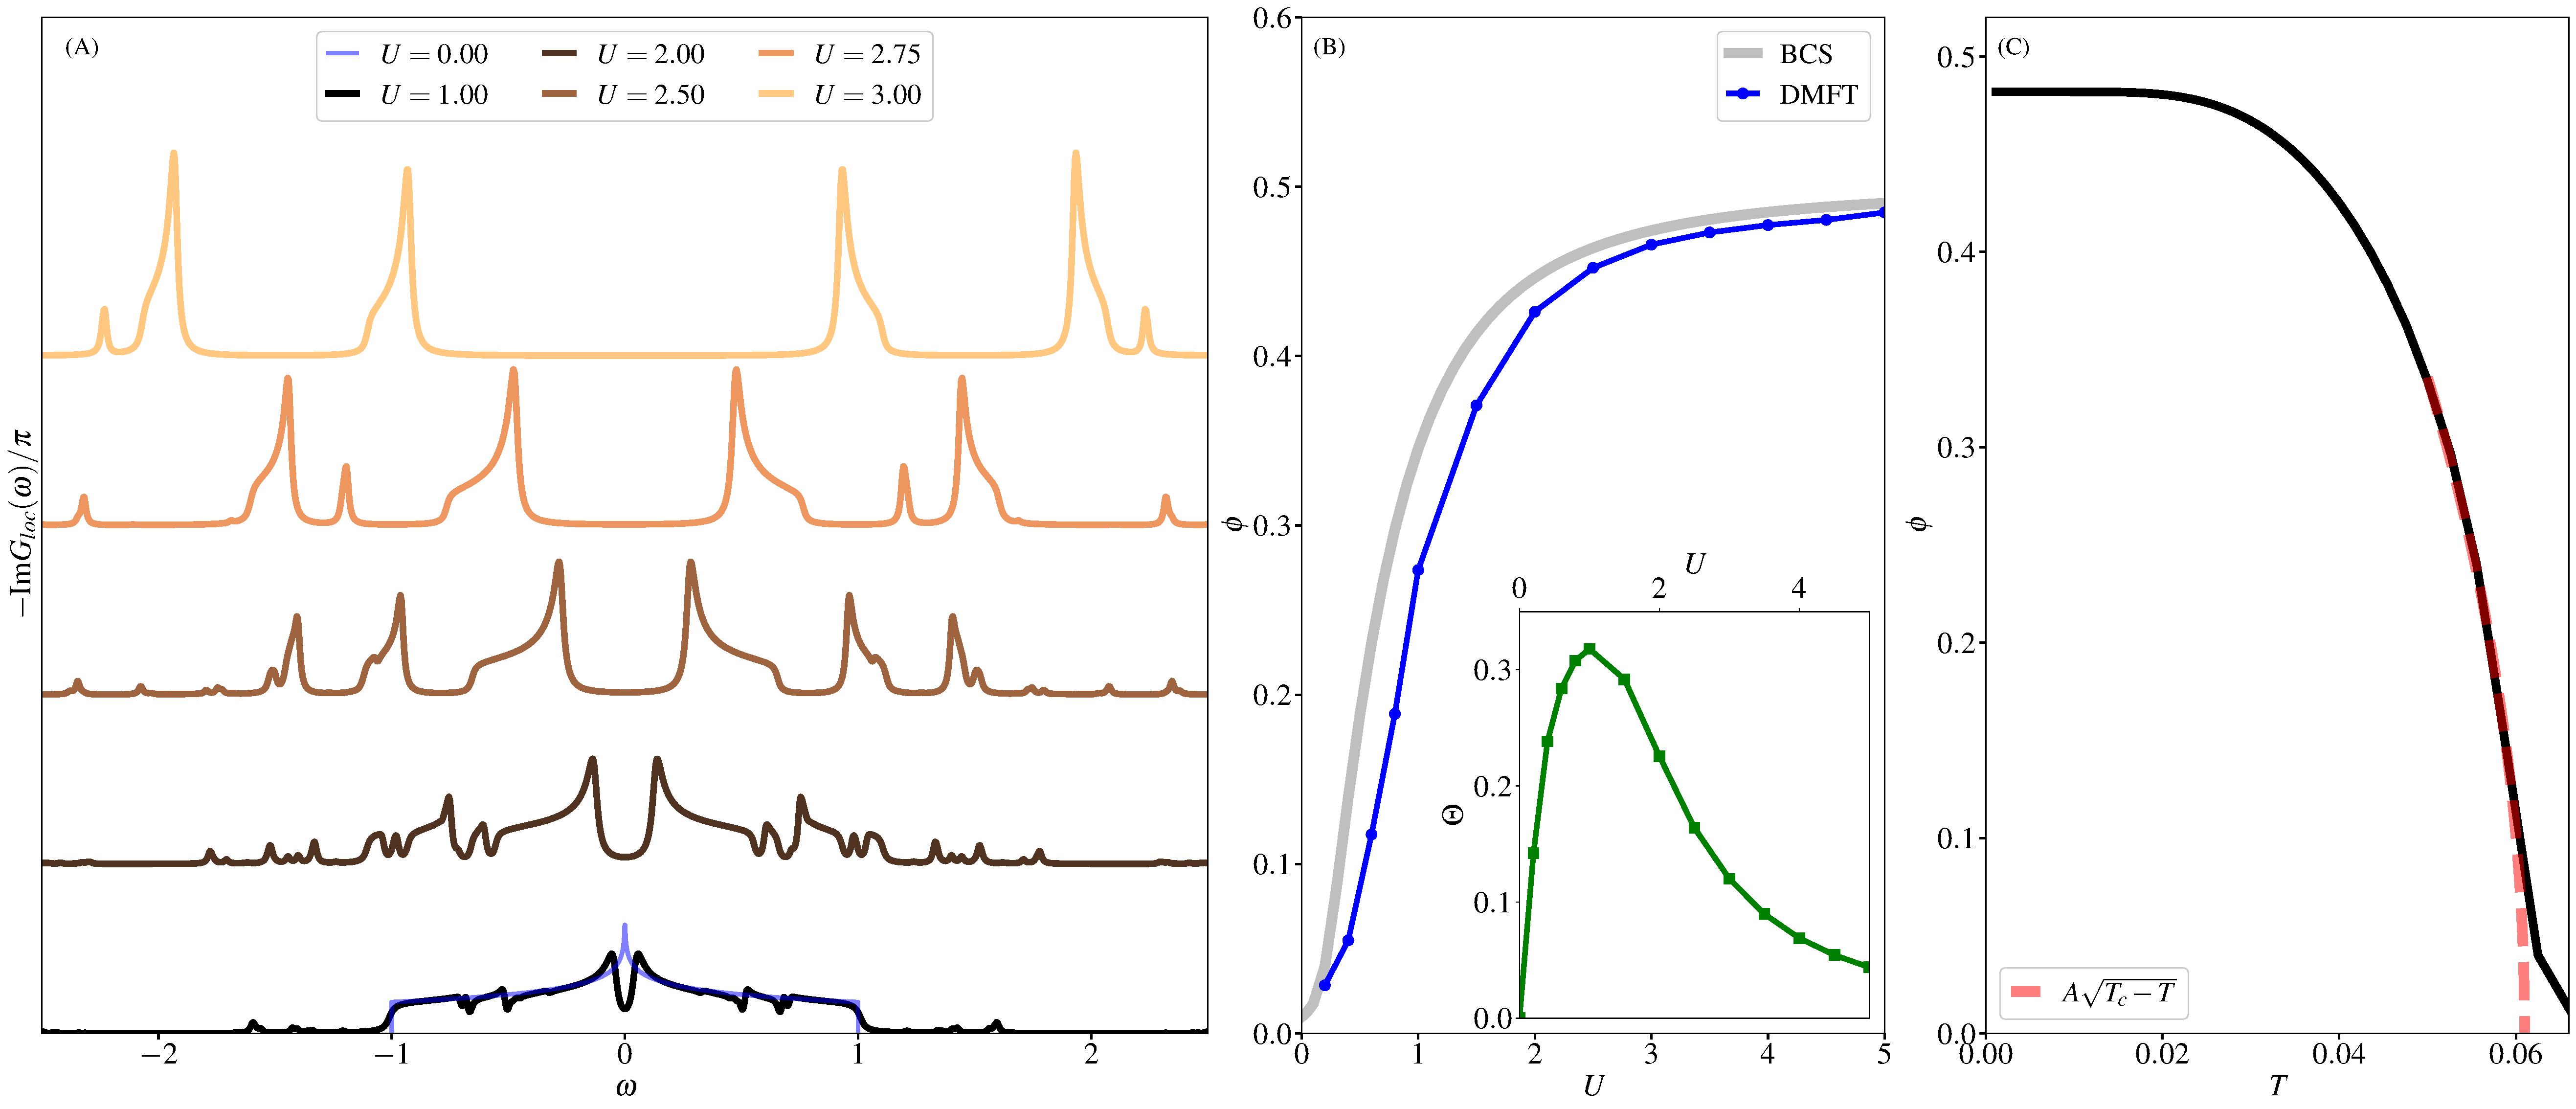
\includegraphics[width=\linewidth]{figures/figAHM.pdf}
    \caption{\label{figEx2}%
      \textbf{The BCS to BEC crossover.}
      (a) Evolution of the spectral functions
      $-\Im{G_\mathrm{loc}(\omega)}/\pi$ as a function of increasing
      attraction $U$. 
      (b) The order parameter $\phi=\langle c_\up c_\dw\rangle$ as a
      function of the attraction $U$. Data for BCS (gray) is compared
      to DMFT results (blue line and symbols). 
      (c) The correlation strength
      $\Theta=\frac{|S(i\omega\to0)-S(i\omega\to\infty)|}{S(i\omega\to\infty)}$ as a function of the
      attraction $U$ across the BCS-BEC crossover. 
      (d) Comparison of the double occupation $D=\langle n_\up
      n_\dw\rangle$ as a function of attraction $U$ between BCS (gray
      solid line) and DMFT (blue solid line and symbols). 
      (e) Superconducting order
      parameter $\phi$ as a function of temperature across the
      superconductor-to-normal phase transition. Data for $U=4$. The
      fit highlights the critical behavior with a mean-field exponent
      $\beta=1/2$ (red dashed line) and parameters $A\simeq 3.7$, $T_\mathrm{c}=0.61$.       
        }
\end{figure}

\paragraph{Results}
Here we showcase some results for the DMFT solution of the 
attractive Hubbard model across the BCS to BEC crossover regime, 
illustrating the capability of \NAME to handle $s$-wave 
superconductivity at both zero and finite temperatures.

To begin, panel (A) of \figu{figEx2} shows the evolution of the 
spectral density, obtained from the local normal Green's function as 
$-\tfrac{1}{\pi}\Im G_\mathrm{loc}(\omega)$, as a function of the 
attraction $U$. For any finite $U$, the Van Hove peak at 
$\omega = 0$ characteristic of the 2D square lattice (visible at 
$U = 0$) is split by the formation of a superconducting gap, whose 
width increases with $U$. This gap reflects the emergence of a finite 
order parameter $\phi = \langle c_\up c_\dw \rangle$, signaling the 
onset of superconducting coherence.


The evolution of this order parameter is presented in panel (B), 
highlighting the crossover from the weak-coupling BCS regime to the 
strong-coupling BEC regime. In the BCS limit, $\phi$ shows the 
characteristic exponential growth with $U$, reflecting the formation 
of weakly bound Cooper pairs. This regime is known to be 
computationally challenging. In the opposite, strong-coupling, limit 
$\phi$ saturates at its theoretical maximum of $\phi \rightarrow 1/2$, 
indicating tightly bound local pairs. Comparison with the mean-field result 
(gray line) reveals the effect of local dynamical fluctuations, which 
slightly suppress the order parameter, particularly in the intermediate 
regime.



To quantify these dynamical effects, we plot in panel (C) the 
\emph{correlation strength}
$\Theta=\frac{|S(i\omega\to 0)-S(i\omega\to\infty)|}{S(i\omega\to\infty)}$
where $S(i\omega)$ is the anomalous self-energy.
This ratio encapsulates, in a single positive number, % sorry, but "statically captures" sounded quite mysterious to me (I guess it refers to having just a single number, but it requires hard mental processing, imho)
the amplitude of the dynamical dependence of $S(i\omega)$ by comparing its 
BCS-like limit at high energy with the low-energy behavior at the Fermi level. 
Large values of $\Theta$ indicate an anomalous self-energy with 
significant dynamical effects, hence a more correlated superconducting state.
Our results show that both the weak 
and strong coupling limits are relatively close to the BCS results, 
while the intermediate regime is marked by strong 
correlations, significantly departing from the mean-field picture.

To further illustrate the impact of dynamical fluctuations, we 
present in panel (D) the evolution of the double occupancy 
$d = \langle n_\up n_\dw \rangle$ as a function of $U$. At half-filling, 
the mean-field expression for this quantity is $d = 1/4 + \phi^2$, 
reflecting the sole contribution of the order parameter. Our DMFT 
results show a slight increase in $d$ over the mean-field prediction 
in the weak coupling regime, corresponding to a steep growth of
the correlation strength $\Theta$. 
However, as $U$ increases, the double occupancy drops below 
the BCS result, reflecting the onset of strong pairing and 
pair localization in the BEC limit. Correspondingly, $\Theta$ 
progressively decreases at large $U$ attraction strength.

Finally, we demonstrate the ability of \NAME to capture finite 
temperature effects. Panel (E) shows the temperature dependence of 
the order parameter $\phi(T)$ across the superconducting-to-normal 
transition. The mean-field nature of this transition is evident from 
the scaling near the critical temperature 
$\phi \sim (T_\mathrm{c} - T)^\beta$ with $\beta = 1/2$, consistent 
with classical Ginzburg-Landau theory.

These results collectively illustrate the versatility of \NAME in 
handling both ground state and finite temperature superconducting 
phases, capturing the complex physics of the BCS-BEC crossover with 
high accuracy.














\begin{figure}[t!]
    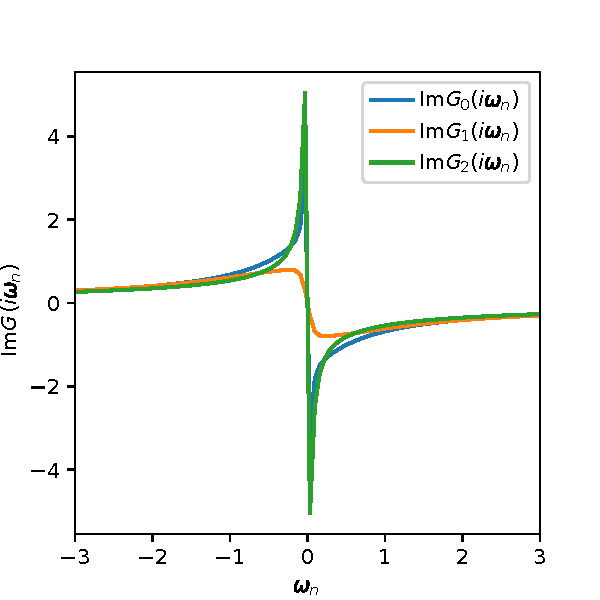
\includegraphics[width=0.5\linewidth]
        {edipack2_examples/edipack2triqs/G_iw.pdf}
    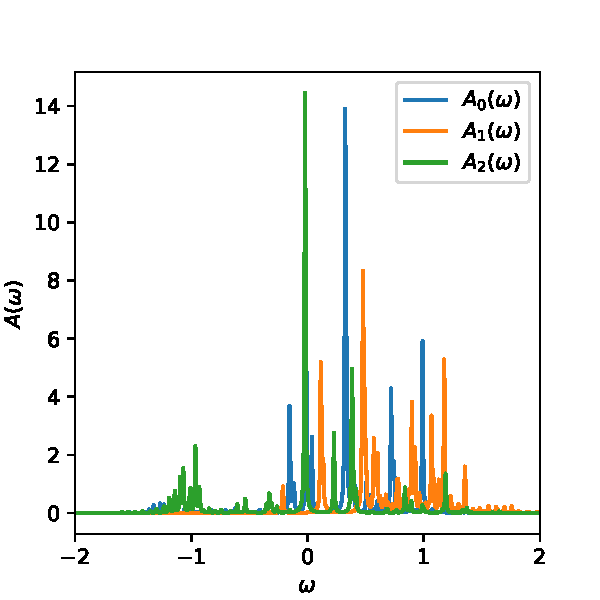
\includegraphics[width=0.5\linewidth]
        {edipack2_examples/edipack2triqs/A_w.pdf}
    \caption{\label{figEx3}%
        Imaginary part of the Matsubara Green's function (left) and the
        corresponding orbital-resolved spectral function (right) computed for a
        three-orbital impurity model with an interaction of the Hubbard-Kanamori
        type (\ref{Hint}). This illustration is produced by the edipack2triqs
        example script presented in Sec.~\ref{SecExamplesTRIQS}.
    }
\end{figure}

\subsection{Multi-orbital quantum impurity with Hubbard-Kanamori
  interaction (TRIQS interface)}
\label{SecExamplesTRIQS}

The third example demonstrates how to use the edipack2triqs compatibility
layer (Sec.~\ref{sSecInteropTRIQS}) to solve a quantum system comprised by a
3-orbital correlated impurity coupled to a few non-interacting bath sites.
The interaction term of the impurity Hamiltonian has the Hubbard-Kanamori
form (\ref{Hint}).

\fixme{Add Hamiltonian?}
\fixme{}


A Python script implementing a calculation that makes use of edipack2triqs
generally begins with a few module imports.
\lstinputlisting[style=mypython,
                 numbers=none,
                 basicstyle={\scriptsize\ttfamily},
                 firstline=1, lastline=13]
{edipack2_examples/edipack2triqs/hubbard_kanamori.py}

One then proceeds to defining the system under consideration. In this case we
consider an impurity atom with three correlated orbitals and two bath states
per each impurity orbital. This information must be encoded in the fundamental
set objects that are later used to construct the solver.
\lstinputlisting[style=mypython,
                 numbers=none,
                 basicstyle={\scriptsize\ttfamily},
                 firstline=15, lastline=26]
{edipack2_examples/edipack2triqs/hubbard_kanamori.py}
The next step is to define a TRIQS many-body operator expression that represents
the Hamiltonian to be diagonalized.
\lstinputlisting[style=mypython,
                 numbers=none,
                 basicstyle={\scriptsize\ttfamily},
                 firstline=28, lastline=67]
{edipack2_examples/edipack2triqs/hubbard_kanamori.py}
Finally, one creates a solver object and performs the actual calculation by
calling its method {\tt solve()}. This is normally the most time- and
memory-consuming step.
\lstinputlisting[style=mypython,
                 numbers=none,
                 basicstyle={\scriptsize\ttfamily},
                 firstline=69, lastline=83]
{edipack2_examples/edipack2triqs/hubbard_kanamori.py}
The computation results are readily available as attributes of the solver
object. The following code snippet shows how to access measured expectation
values of the static observables, and how to employ the plotting framework of
TRIQS to visualize the obtained Matsubara and real-frequency impurity Green's
functions (Fig.~\ref{figEx3}).
\lstinputlisting[style=mypython,
                 mathescape=false,
                 numbers=none,
                 basicstyle={\scriptsize\ttfamily},
                 firstline=85, lastline=112]
{edipack2_examples/edipack2triqs/hubbard_kanamori.py}














\subsection{Interacting Bernevig-Hughes-Zhang model (Fortran API, {\tt ed\_mode=nonsu2})}
In this section we focus on the DMFT solution of the interacting
Bernevig-Hughes-Zhang (BHZ).
As shown in Ref.~\onlinecite{AmaricciPRB2022}, at moderate
interactions this model admits an excitonic phase in which opposite
orbitals electrons and holes across the band gap bound into a coherent phase.

We consider a system of two-orbital electrons on a square
lattice interacting through a Hubbard-Kanamori term and describing
a quantum spin Hall insulator.
We consider a suitable matrix basis in terms of the Dirac
matrices $\Gamma_{a\a}=\sigma_a\otimes \tau_\a$, where $\sigma_a$ and
$\tau_\a$ are Pauli matrices, respectively, in the spin and orbital
pseudo-spin space. The  model Hamiltonian reads
$$
H = \sum_{k}\psi_{k}^\dagger H(k)\psi_{k} + H_{\rm int}
$$
where $\psi_{k}=[c_{1\uparrow k}, c_{2\uparrow k},
c_{1\downarrow k}, c_{2\downarrow k} ]$ is the spinor collecting
annihilation operator $c_{a\sigma k}$ destructing an electrons at
orbital $a=1,2$ with spin  $\sigma=\up,\dw$ and lattice momentum
$k$. The non-interacting part of the Hamiltonian is:
$$
H(k) = \left[M-2t(\cos{k_x}+\cos{k_y}) \right]\Gamma_{03} +
   \lambda\sin{k_x}\Gamma_{31} -   \lambda\sin{k_y}\Gamma_{02}
$$
where $M$ is the mass term, which plays the role of a crystal
field splitting among the orbitals. The presence of this term breaks
the symmetry in the orbital pseudo-spin channel.
The  interaction reads: 
$$
   H_{\rm int} = (U-J)\frac{\hat{N}(\hat{N}-1)}{2} - J\left( \frac{1}{4}\hat{N}^2 +
   \hat{S_z}^2 - 2 \hat{T_z}^2\right)
 $$
 where $\hat{N}=\tfrac{1}{2}\psi_i^\dagger \Gamma_{00}\psi_i$ is the
total density operator,
$\hat{S_z}=\tfrac{1}{2}\psi_i^\dagger \Gamma_{30}\psi_i$ is the total
spin polarization operator and $\hat{T_z}=\tfrac{1}{2}\psi_i^\dagger
\Gamma_{03}\psi_i$ is the orbital pseudo-spin polarization operator.
This form corresponds to the density-density part of the
Kanamori interaction. We neglect the pair-hopping and spin-flip purely
for numerical reasons. 

In the non-interacting regime, i.e. $U=J=0$ this model describes a
quantum spin Hall insulator (QSHI) for $M<4t$ and a trivial Band
Insulator (BI) for $M>4t$.
The transition point at $M=4t$ describes the formation of a gapless
Dirac state with linear band crossing at $k=[0,0]$.  


The code implementation follows the same guidelines discusses above
for the other examples. There are two specific modifications requied
to the  user. The first is to generate the Hamiltonian $H(k)$ on a discretized Brillouin zone in
order to obtain the local interacting Green's function, used in the
implementation of the self-consistency conditions:
$\GG^{-1}=G_{loc}^{-1}+\Sigma$, with: 
$$
G_{loc}(z) = \tfrac{1}{N_k}\sum_k \left[z+\mu-H(k)-\Sigma(z)
\right]^{-1}, 
$$
where $\z\in\CCC$  and $\Sigma(z)$ is the self-energy function obtained from the DMFT
solution of the proble.  $N_k$ is the number of $k$-points. 
The second is to  construct the ``renormalized'' topological
Hamiltonian
$$
H_{top} = \sqrt{Z}[H(k) + \Re\Sigma(\omega\to0)]\sqrt{Z}, 
$$
where $Z$ is the renormalization constant. $H_{top}$ describes the
low-energy properties of many-body problem and can be used to obtain a 
topological characterization of the interacting system.  



\begin{figure}[t!]
  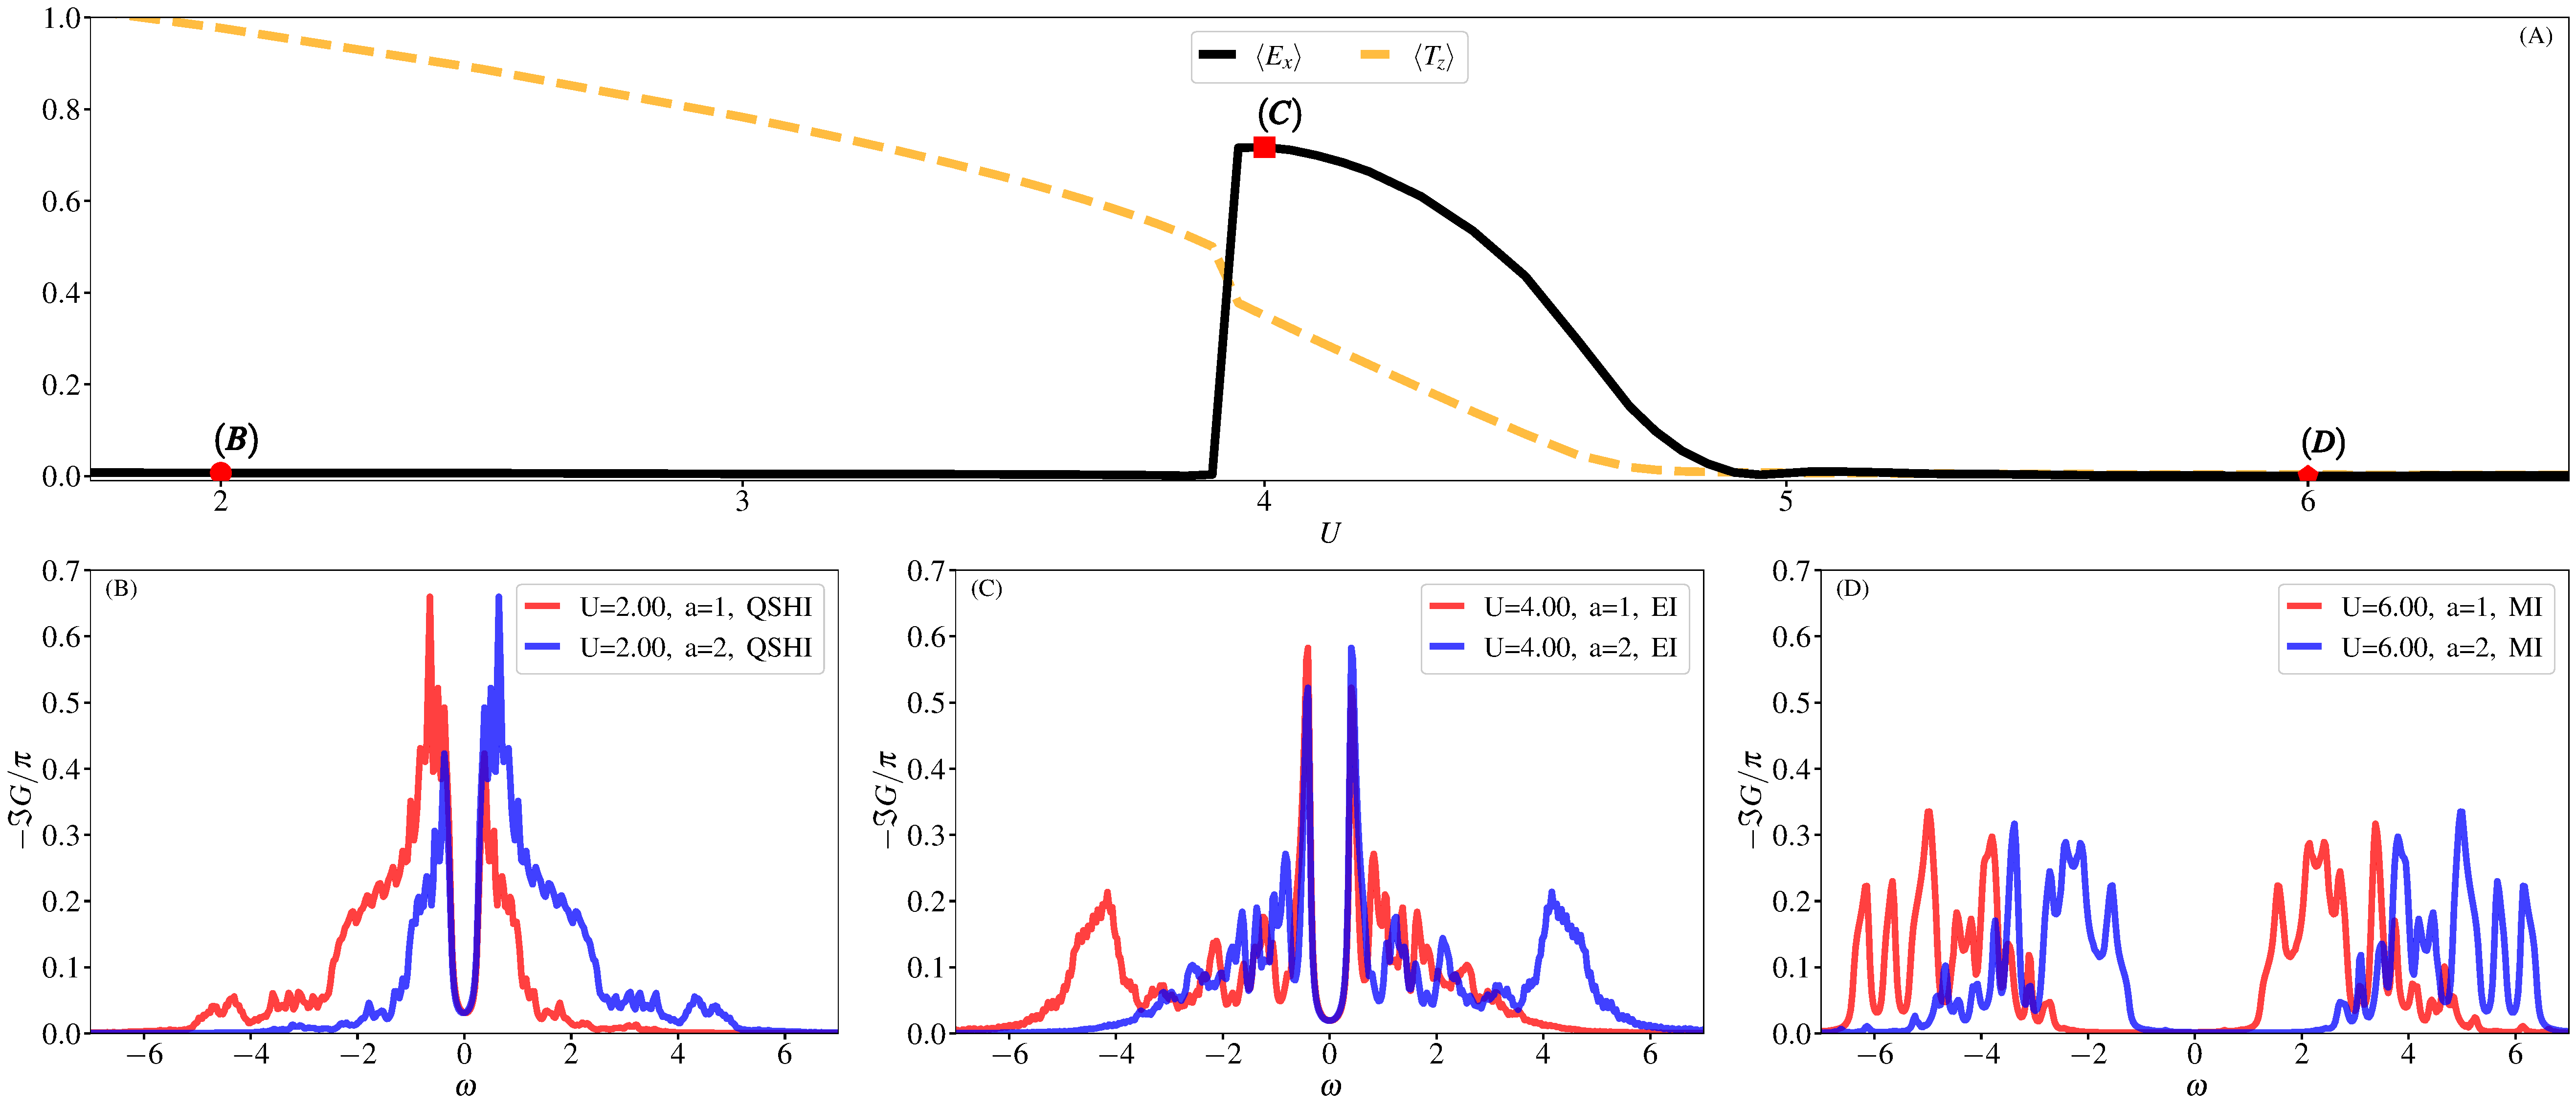
\includegraphics[width=\linewidth]{figures/figBHZ.pdf}
    \caption{\label{figEx4}%
      \textbf{Topological and Exciton Transition.}
      (A) Evolution of the spin-triplet,
      in-plane excitonic order parameter $\langle E_x\rangle$ (black solid line) and
      orbital polarization $\langle T_z\rangle$ (orange dashed line) as a function of the
      interaction $U$.
      (B-D) Spectral functions of the two orbital electrons for three
      values of the interaction $U=2.00$ (red circle), $4.00$ (red
      square) and $6.00$ (red diamond) capturing, respectively, the
      QSHI (B), the Excitonic Insulator (C) and the Mott Insulator
      (D). 
    }
\end{figure}

\paragraph{Results}
To capture the possible symmetry breaking in any excitonic channel
driven by the local interaction, we consider the vector order
parameter
$\vec{E}=[E_0,E_x,E_y,E_z]$ where $E_a=\langle\psi^\dagger
\Gamma_{a1}\psi \rangle$.
The first component $E_0$ describes the singlet excitonic state,
whereas the remaing ones correspond to the triplet states with
different spin orientation.   
The analysis of the strong-coupling regime as well as impurity
excitonic susceptibility available in \NAME suggest the possible
instability to an in-plane spin-triplet exciton phase, i.e. with $E_x$
and/or $E_y$ different from zero.
Interestingly, this state breakes several symmetries including
time-reversal and spin SU(2) which protect the topological state.

Thus, here we illustrate the DMFT solution of the excitonic phase as a way to
illustrate the ability of \NAME to capture matter phases with broken
spin-symmetry ({\tt ed\_mode=nonsu2}) and the use of {\tt
  bath\_type=replica}.
\begin{lstlisting}[style=fstyle,numbers=none,basicstyle={\scriptsize\ttfamily}]
   !> Set $H_{loc}$
   allocate(Hloc(Nso,Nso))
   Hloc = sum(Hk,dim=3)/Lk
   where(abs(dreal(Hloc))<1d-6)Hloc=zero
   call ed_set_hloc(Hloc)
   !> Setup the replica bath basis:
   allocate(lambdasym_vector(Nbath,4))
   allocate(Hsym_basis(Nso,Nso,4))
   Hsym_basis(:,:,1)=Gamma03  ;lambdasym_vector(:,1)= Mh
   Hsym_basis(:,:,2)=Gamma01 ;lambdasym_vector(:,2)= sb_field
   Hsym_basis(:,:,3)=Gamma31 ;lambdasym_vector(:,3)= sb_field
   Hsym_basis(:,:,4)=Gamma11 ;lambdasym_vector(:,4)=-sb_field
   !> Set the replica bath
   call ed_set_Hreplica(Hsym_basis,lambdasym_vector)
   !> Get bath dimension and allocate user bath to this size
   Nb=ed_get_bath_dimension(4)   !There are 4 symmetries
   allocate(Bath(Nb))
   !
   !> Initialize the ED solver (bath is guessed or read from file) 
   call ed_init_solver(bath)
\end{lstlisting}
where we use the local non-interacting Hamiltonian 
$H_{loc}=\tfrac{1}{N_k}\sum_k H(k)$ to set 
$h^0_{\a\b\s\s'}$, i.e. the impurity Hamiltonian. To anticipate the
possibility of forming an excitonic ordered phase, the replica bath
is constructed out of matrix basis with 4 distinct elements
$\Gamma_{03}$, $\Gamma_{01}$, $\Gamma_{31}$, $\Gamma_{11}$ which
are proportional, respectively, to the mass term, the exciton singlet
$E_0$, the exciton triplet along easy-axis $E_z$ and in-plane
$E_x$ (we assume $E_y=0$ levaraging on residual $U(1)$ in-plane
symmetry. 




In the following we consider the case of $M=1$ which corresponds to a
QSHI in the non-interacting limit and $J/U=0.25$.
The implemention is nearly identical to the cases discussed above and
we report it here for completeness:
\begin{lstlisting}[style=fstyle,numbers=none,basicstyle={\scriptsize\ttfamily}]
   iloop=0;converged=.false.
   do while(.not.converged.AND.iloop<nloop)
     iloop=iloop+1
     !> Solve the impurity problem, retrieve $\Sigma(i\omega)$
     call ed_solve(bath)
     call ed_get_sigma(Smats,axis='mats')
     !> Get $G_{loc}$ (assume to have a function for this task)
     call get_gloc(Hk,Gmats,Smats,axis='m')
     !> Update the Weiss field $\GG^{-1}=G^{-1}_{loc}+\Sigma$ +  Linear mixing.
     call dmft_self_consistency(Gmats,Smats,Weiss)
     if(iloop>1)Weiss = wmixing*Weiss + (1.d0-wmixing)*Weiss_;Weiss_=Weiss
     !> Fit to updated the bath
     call ed_chi2_fitgf(Weiss,bath,ispin=1)
     !Check convergence (using DMFT_TOOLS)
     converged = check_convergence(Weiss(1,1,:),dmft_error,nsuccess,nloop)
   enddo  
\end{lstlisting}

%
The main effect of the interaction is enclosed in the renormalized
mass term $M_{eff}=M+\tfrac{1}{4}\Tr{\Re\Sigma(i\omega\to0)}$. The
real-part of the self-energy being proportional to $\Gamma_{03}$
corrects the mass term with respect to its bare value. To leading
order this correction is given proportional to $\tfrac{U-5J}{4}\langle
\hat{T}_z\rangle$. So, for our choice of parameters, the effect of
interaction would be to reduce the (effective) mass term and thus
reducing the topological band gap. In the strong-coupling limit the
two orbitals get populated with one electron per site, reaching the
conditions for the formation of a Mott insulating state.
As reported in panel (A) of \figu{figEx4}, at intermediate coupling,
the DMFT solutions features the formation of a
region of exciton condensation with $\langle E_x\rangle>0$, $\langle
E_0\rangle=\langle E_z\rangle=0$. 
Unlike the static mean-field description~\cite{Blason}, the
transition from the QSHI topological state to the Excitonic Insulator 
(EI) becomes of first-order in presence of quantum fluctuations
corrections~\cite{Continentino,Paoletti} contained in DMFT. On the
other hand, the EI continuously evolves into a Mott Insulator (MI)
for larger interaction (neglecting for simplicity any 
anti-ferromagnetic ordering that would naturally occurr in this
regime).
In the same panel we report the evolution of 
$\langle T_z\rangle$ to illustrate the progressive reduction of the
orbital polarization and, thus, of the effective mass. 


To further illustrate the nature of the three distinct phases of this
system, we leverage on the direct access to real-axis spectral
function provided by \NAME solver. In panels (B)-(D) of \figu{figEx4}
we report the spectral functions $-\Im{G}_{a,loc}(\omega)/\pi$ for
$a=1,2$, $\sigma=\up$ and three distinct values of the interaction
$U$ placing the solution, respectively, in the QSHI, the EI and the MI.
The correlated QSHI is characterized by the presence of an 
inverted band gap featuring a substantial orbital spectral mixing. The
EI spectrum is instead characterized by a narrow gap, related to the
finite order parameter, flanked by two sharp resonances and featuring
larger high-energy weight.
Finally, in the MI the two orbital spectral function describes the two 
characteristic Hubbard bands separated by a large Mott gap.  






\subsection{Holstein model on the Bethe lattice (Fortran API, {\tt electron-phonons})}
One of the features introduced in \NAME is the possibility of treating
local phonons in conjunction with the superconductive phase,
i.e. \textbf{ed\_mode=superc}. 
In this example discuss  the normal and
superconductive solution of the pure Holstein model on the Bethe
lattice within DMFT.
We stress that, using Fortran API, the code
implementation for this specific case is essentially identical to the listing reported in the sections
\ref{SecExamplesBetheDMFT} ({\tt ed\_mode=normal}) and
\ref{SecExamplesAHM} ({\tt ed\_mode=superc}). 

So we consider the model introduced in \secu{SecExamplesBetheDMFT}
with $U=0$ and the additional phononic and electron-phonon terms:
\begin{equation} \label{eqex:H_Holstein}
    H_{int} = \sum_i \Big[\omega_0 b^\dagger_i b_i + g(b^\dagger_i +
    b_i)\sum_{\sigma}(c^\dagger_{i\sigma}c_{i\sigma}
    -\frac{1}{2})\Big]. 
\end{equation}
We consider the half-filling regime of the particle-hole symmetric
Bethe lattice density of states. We set the half-bandwidth as our
energy unit $D=1$ and introduced the electron-phonon coupling $\lambda
= \tfrac{2g^2}{\omega_0D}$.  
The iterative DMFT solution algorithm follows the same principles
illustrated in the previous sections. 

\paragraph{Results}
In the following we discuss the adiabatic ($\omega_0\to0$) to
anti-adiabatic ($\omega_0\to\infty$) crossover for
the uniform solution of the Holstein model at constant coupling $\lambda=1.0$.

In the anti-adiabatic limit, the Holstein interaction takes a
particularly simple form:
\begin{equation}\label{HlikeAttraction}
    H_{int} \overset{ \omega_0 \rightarrow \infty}{ \longrightarrow } -\frac{\lambda}{2} \sum_i \Big[\sum_\sigma(c^\dagger_{i\sigma}c_{i\sigma} -\frac{1}{2}) \Big]^2
\end{equation}
which describes a local Hubbard-like attraction among electrons
(mediated by local phonons).
In the opposite, adiabatic, limit, $\omega_0 \rightarrow 0$ the system
enters in a Bipolaronic Insulating phase~\cite{Capone2006PRB} for our
choice of the coupling. 


We characterize the model solution by showin the evolution of the
double occupation $\langle n_{\up}n_{\dw}\rangle$ as a function of the
phonon frequency $\omega_0$, see panel (A). In this panel we compare
the behavior for {\tt ed\_mode=normal} against the superconductive
solution ({\tt ed\_mode=superc}). Our results capture the whole
crossover from adiabatic to anti-adiabatic regime. In the former
regime, the double occupation takes a similar value for the two
phases. However, approaching the anti-adiabatic regime, the two
solutions reach the limiting values corresponding to the residual
attraction \equ{HlikeAttraction}.   
To better characterize the nature of the superconducting
phase in the Holstein model we report the evolution of the anomalous order
parameter $\phi$ in the adiabatic to anti-adiabatc crossover.
The DMFT results obtained with \NAME show the rapid increase of the
superconducting order parameter as phonon frequency grows
large. Finally, in the anti-adiabatic regime $\phi$ saturates to a
finite value corresponding to the attractive Hubbard-like interaction
of strenght $\lambda/2$. 

\begin{figure}[ht!]
    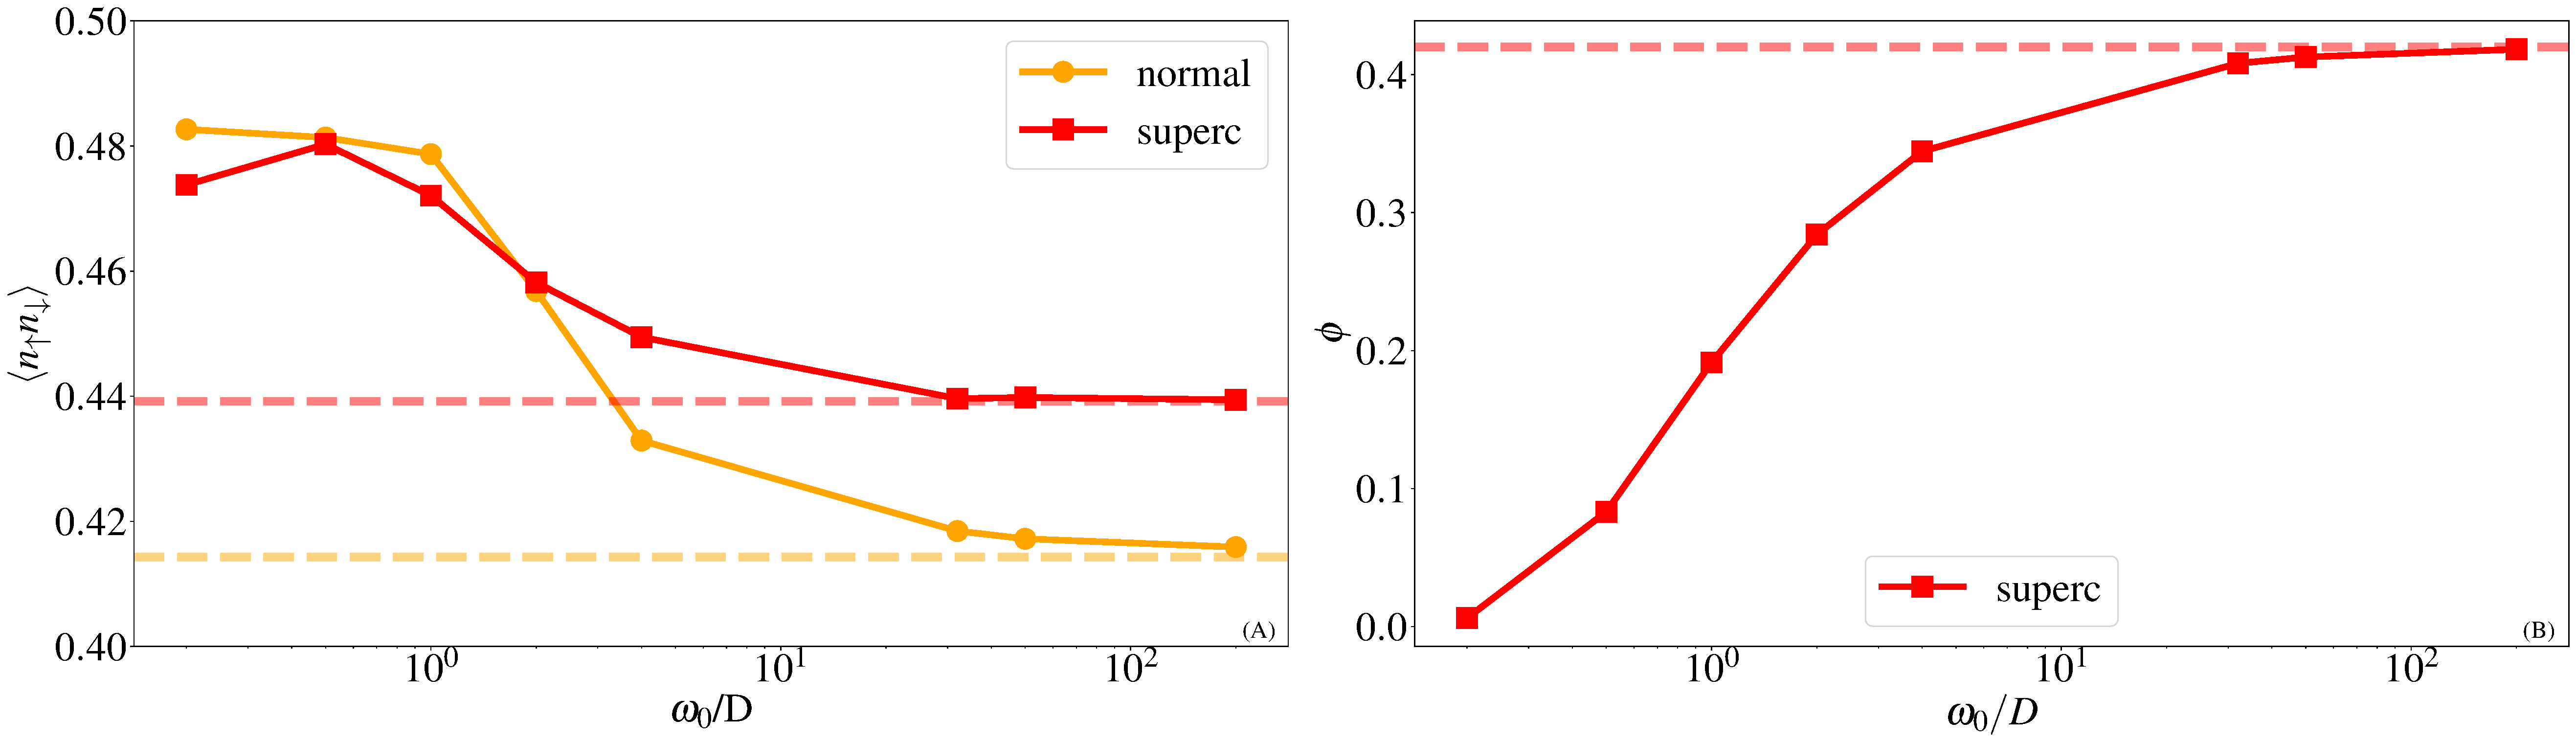
\includegraphics[width=\linewidth]{figures/figBethe_Holstein.pdf}
    \caption{\label{figEx5}
      Evolution of the  double occupation (A) and superconductive order parameter (B) as a function of $\omega_0/D$ for $\lambda=1$ in the normal (orange) and superconductive (red) phase. The horizontal broken line are the values for the corresponding Hubbard model in the anti-adiabatic limit.}
\end{figure}




\end{document}
